\documentclass[12pt]{article}
\usepackage{graphicx} % This lets you include figures
\usepackage{hyperref} % This lets you make links to web locations
\graphicspath{ {./images/} }

\usepackage[rightcaption]{sidecap}
\usepackage{caption}
\usepackage{subcaption}
\usepackage{hyperref}

\usepackage{float}

\usepackage{imakeidx}

\usepackage{tikz}
\usetikzlibrary{shapes.geometric, arrows}
\tikzstyle{startstop} = [rectangle, rounded corners, minimum width=3cm, minimum height=1cm,text centered, draw=black, fill=red!30]
\tikzstyle{io} = [trapezium, trapezium left angle=70, trapezium right angle=110, minimum width=3cm, minimum height=1cm, text centered, draw=black, fill=blue!30]
\tikzstyle{process} = [rectangle, minimum width=3cm, minimum height=1cm, text centered, draw=black, fill=orange!30]
\tikzstyle{decision} = [diamond, minimum width=3cm, minimum height=1cm, text centered, draw=black, fill=green!30]
\tikzstyle{arrow} = [thick,->,>=stealth]

\usepackage{todonotes}

\usepackage{amsmath,amssymb}
\let\amssymbboxplus\boxplus
\let\amssymbboxminus\boxminus

\renewcommand{\boxplus}{\mathbin{\mathop\amssymbboxplus}}
\renewcommand{\boxminus}{\mathbin{\mathop\amssymbboxminus}}

\makeindex


\title{Computer and network security}
\author{Beau De Clercq}
\date{2020-2021}

\begin{document}
	
 \maketitle{}
 
 \tableofcontents
 
 \clearpage
 \newpage
 
 \section{Introduction}
 
 \section{Symmetric ciphers}
 
 \section{Message authentication}
 \subsection{Hash functions}
 A hash function H is a function that takes input data blocks of length M and returns a hash value of fixed size R.\\
 A cryptographic hash function that also satisfies following conditions:
 \begin{itemize}
 	\item One way property: it should be infeasible to find a data object that maps to a predefined hash value.
 	\item Collision free property: it should be infeasible to find 2 data objects that map to the same hash value.
 	\item Use padding to pad up input to fixed length and add the length l of the block in bits. 
 \end{itemize}
By satisfying the first two properties, hash functions can  be used to determine if data has been altered.
\subsubsection{Applications}
Hash functions can be used in an number of applications:
\begin{itemize}
	\item Message authentication: to ensure a message hasn't been altered.
	\item Digital signatures: ensure the authenticity of messages and identity of the sender.
	\item One-way password file: store hash value of password in plain text file.
	\item Intrusion/virus detection: store H(f) for each file to determine if files have been modified.
	\item Pseudorandom function: use H to generate pseudorandom private key.
\end{itemize}
\subsubsection{Security requirements}
Cryptographic hash functions must adhere to following security requirements:
\begin{itemize}
	\item Basic:
	\begin{itemize}
		\item Input data can be of any size
		\item Output is of fixed length
		\item H(x) is easy to compute
	\end{itemize}
	\item Advanced:
	\begin{itemize}
		\item Given h, it is hard to find y: H(y) = h
		\item It is hard to find y: y$\ne$x $\&$ H(y)=H(x)
		\item It is hard to find (x, y): H(x)=H(y)
	\end{itemize}
\end{itemize}

\subsubsection{Attacks}
\begin{itemize}
	\item \underline{Brute force preimage attack}\\
	The goal of this attack is to find a y such that H(y) = h for a given hash value h.\\
	The attack itself goes as follows:\\
	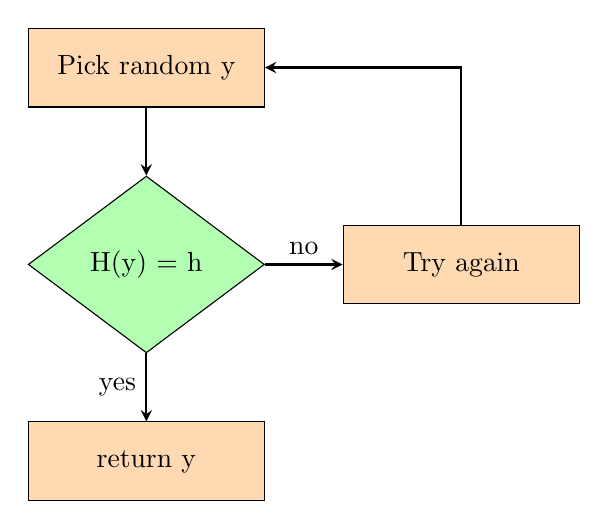
\begin{tikzpicture}[node distance=2cm]
	
	\node (pro1) [process] {Pick random y};
	\node (dec1) [decision, below of=pro1, yshift=-0.5cm] {H(y) = h};
	\node (pro2a) [process, below of=dec1, yshift=-0.5cm] {return y};
	\node (pro2b) [process, right of=dec1, xshift=2cm] {Try again};

	\draw [arrow] (pro1) -- (dec1);
	\draw [arrow] (dec1) -- node[anchor=east] {yes} (pro2a);
	\draw [arrow] (dec1) -- node[anchor=south] {no} (pro2b);
	\draw [arrow] (pro2b) |- (pro1);

	\end{tikzpicture}\\
	On average this attack need $2^{m-1}$ attempts for an m-bit hash value.
	\item \underline{Brute force collision resistance attack}\\
	The goal of this attack is to find two values x and y such that H(x) = H(y). This attack need $2^{\frac{m}{2}}$ attempts for an m-bit hash value.\\
	\todo[inline]{Add image of attack from slides}
\end{itemize}
 
 \subsection{Secure Hash Algorithm (SHA)}
 \todo[inline]{Add SHA overview from slides}
 \subsubsection{SHA512}
 \todo[inline]{Add image from slides}
 \subsubsection{SHA512 block processing}
 \todo[inline]{Add image from slides}
 \todo[inline]{Add image of round function from slides}
 In this 80 round process, a message of 1024 bits is transformed into 80 values of 64 bits each which are then individually processed in sequence by means of a round function.\\
 After the final round a word-by-word addition 64-bit words mod$2^{64}$ is performed to obtain the final hashed value.
 \subsubsection{Message schedule}
 The first 16 words $W_0 .. W_{15}$ are derived directly from the input block $M_i$. All other words are derived as follows:
 \begin{align*}
 	W_t = W_{t-16} \boxplus \delta_0(W_{t-15}) \boxplus W_{t-7} \boxplus \delta_1(W_{t-2})\\
 	\delta_0(x) = ROTR^1(x) \oplus ROTR^8(x) \oplus SHR^7(x)\\
 	\delta_1(x) = ROTR^{19}(x) \oplus ROTR^{61}(x) \oplus SHR^6(x)\\
 	ROTR^n(x) = \text{circular right bit-shift by n bits}\\
 	SHR^n(x) = \text{right bit-shift of x by n bits with}\\
 	 \text{padding by n zeros on the left}
 \end{align*}
 
 \subsection{Length extension attack and SHA3}
 \subsubsection{Length extension attack}
 Type of attack where an attacker can use H($M_1$) and the length of $M_1$ to calculate H($M_1|M_2$) for an attack controlled message $M_2$ without needing to know the content of $M_1$. This is done by taking the old message and using it as 'intermediary' input in the hashing algorithm.
 \subsubsection{SHA3}
 \todo[inline]{Add image from slides}
 
 \subsection{Message authentication}
 There are 8 types of attacks:
 \begin{enumerate}
 	\begin{multicols}{2}
 		\item Disclosure of message content
 		\item Traffic analysis
 		\item Masquerade
 		\item Content modification
 		\item Sequence modification
 		\item Timing modification
 		\item Source repudiation
 		\item Destination repudiation
 	\end{multicols}
 \end{enumerate}
 Items 1 and 2 can be countered using confidentiality mechanisms, eg symmetric encryption.\\
 Items 3 to 6 can be countered by using \underline{message authentication} to verify that the received message hasn't been altered.\\
 \underline{Digital signatures} can be seen as an extension to message authentication as it is an authentication technique that also includes measures to counter repudiation by the source.\\
 \newline
 A message authentication function is a function that produces an authenticator (a value to be used to authenticate a message). There are 3 classes of message authentication functions:
 \begin{itemize}
 	\item Hash functions:
 	\begin{itemize}
 		\item Concatenate message M with secret key S and hash the stream
 		\item Send message M together with hash value: if it is intercepted an attacker can't create a new hash value since the key is unknown
 		\item Check authentication: combine M with S, hash the stream and compare with received hash value
 	\end{itemize}
 	\item Message encryption, eg using symmetric encryption, provides both confidentiality and authentication if key K is secret. If the decrypted message M is not meaningful then the message can be considered altered.
 	\item Message authentication code (MAC): generates fixed-size cryptographic checksum based on message and secret key
 	\begin{itemize}
 		\item Does not need to be reversible
 		\item send message with checksum: if the checksum calculated by the receiver doesn't match then the message has been altered
 		\item Cannot be used to provide digital signatures: a signature need to be verifiable by anyone and MAC requires the use of a secret key
 	\end{itemize}
 \end{itemize}
 \subsubsection{Security requirements for MAC}
 \begin{itemize}
 	\item If an opponent observes $M$ and $MAC(K, M)$, it should be infeasable to construct $M'$ such that $MAC(K, M') == MAC(K, M)$.
 	\item Given 2 randomly chosen messages $M$ and $M'$, the probability that $MAC(K, M) == MAC(K, M')$ should be $2^{-N}$ for an N-bit code. $-->$ codes should be distributed uniformly and random over the entire output space
 	\item If $M'$ is a known transformation of $M$, then $\mathbb{P}(MAC(K, M) = MAC(K, M') = 2^{-N}$.
 \end{itemize}

 \subsection{Message authentication codes}
 \subsubsection{Cipher-based MAC (CMAC)}
 \begin{itemize}
 	\item $M$ is split into fixed size blocks $M_1, ..., M_N$.
 	\item $M_1$ is encrypted with key $K$ of k bits.
 	\item Resulting block is then XORed with next input block, the result is then encrypted with the same key $K$. This process is repeated until block $M_{N-1}$.
 	\item At the final block $M_N$: XOR $M_N$ with $M_{N-1}$ and b-bit constant $K_1$ derived from the original key.
 	\item Encrypt the result using key $K$, then the leftmost significant bits represent the tag.
 	\item If $M$ is not a multiple of b: last block is padded with $10..0$ and $K_2$ is used in stead of $K_1$.
 	\item Determining $K_1$ and $K_2$: 
 	\begin{equation*}
 		L = E(K, 0^b), K_1 = L*x, K_2 = L*x^2 
 	\end{equation*}
 	where multiplication happens in $GF(2^b)$
 \end{itemize}
 
 \subsubsection{Hash-based MAC (HMAC)}
 \begin{itemize}
 	\item Advantages: hash functions execute faster and library code is widely available.
 	\item Main issue: a secret key needs to be used when using a hash function.
 	\item Objectives:
 	\begin{itemize}
 		\item To use, without modification, available hash functions;
 		\item To allow for easy replaceability of the hash function;
 		\item To preserve the hash function's original performance;
 		\item To use and handle keys in a simple way;
 		\item To have a well understood cryptographic analysis.
 	\end{itemize}
 	\item Structure: \todo[inline]{copy image from slide}
 	\item Cryptographic strengths:
 	\begin{itemize}
 		\item HMAC can be proven secure provided that the embedded hash function has some reasonable cryptographic strengths.
 		\item A successful attack on HMAC is equivalent to one of the following:
 		\begin{itemize}
 			\item The attacker is able to compute an output of the compression function.
 			\item The attacker finds collisions in the hash function.
 		\end{itemize}
 	\end{itemize}
 \end{itemize}

 
 \section{Asymmetric encryption}
 
 \section{Key distribution}
  
\end{document}